\chapter{Описание программного обеспечения устройства}
\hspace{1cm} 

Для реализации основной функциональности отладчика был модифицирован исходный код проекта 
Blackmagic \cite{BlackMagic}. Этот проект представляет открытую (под лицензией GPL) реализацию протокола 
отладчика GDB (GNU Debug), ориентированную для работы с микроконтроллерами на ядре Cortex-M и RISC-V. 
Так как целевой платформой для Blackmagic являются, в том числе, различные микроконтроллеры 
семейства STM32, первоначальное портирование ПО отладчика на STM32F107 свелось к редактированию 
конфигурационных файлов.

Следующей задачей стала реализация управления отладчиком по TCP. Так как отладчик GDB предназначен 
в том числе для работы с удаленными системами, его протокол управления для подключения к ним может
работать не только поверх последовательного порта (или, как в оригинальном Blackmagic, его реализации
поверх USB), но и поверх TCP-соединений. В качестве реализации протоколов семейства TCP/IP была 
выбрана библиотека lwIP \cite{LWIP:doc}, предназначенная в том числе для встраиваемых систем.

lwIP предполагает несколько вариантов использования, так как в оригинальном ПО Blackmagic 
отсутствует поддержка многозадачности, был выбран режим с периодическим вызовом функций lwIP 
из главного цикла приложения -- Mainloop mode, или NO\_SYS в терминологии документации 
lwIP. \cite{LWIP:doc}.

Реализация работы с протоколом GDB в Blackmagic используются функции gdb\_if\_putchar для отправки 
данных и gdb\_if\_getchar/gdb\_if\_getchar\_to для их получения. Последняя пара функций регулярно 
вызывается из главного цикла приложения, что позволяет добавить в них необходимые вызовы функций lwIP. 
Работа с буферами данных для интерфейса GDB осуществляется из callback-функций, обслуживающих 
соединение по протоколу TCP (порт 3333, как наиболее часто используемый при работе с GDB).

Следует отметить, что протокол отладчика GDB \cite{GDB} не вполне подходит для работы по TCP. 
В частности, передача подтверждения или ошибки обработки сообщения 
- это короткие с точки зрения TCP пакеты, с 1 байтом полезной нагрузки (символ + или -). 
Это обстоятельство вместе с реализованным в lwIP алгоритмом TCP Delayed ACK требуют отключения 
алгоритма Нейгла \cite{RFC Neiqel}, приводящим к задержкам при передаче данных в подобных ситуациях.

Кроме того, для передачи данных от последовательного порта отлаживаемого устройства был реализован
мост TCP-UART (порт 20000, по аналогии с используемым в FIT IoT-LAB шлюзом на базе одноплатного 
компьютера Raspberry PI).

Для мониторинга энергопотребления был адаптирован исходный код проекта Energymon \cite{Energymon Code}, 
распространяющийся под лицензией ISC. Используется встроенный в микроконтроллер аналого-цифровой
преобразователь (АЦП). При первоначальной калибровке определяются показания АЦП при нулевом токе на 
каждом из переключаемых диапазонов шунтов. Эти данные используются для пересчета отсчетов АЦП в 
потребляемый ток (как показано ранее, вносимая при переключении шунтов ошибка влияет в основном на 
смещение передаточной функции вверх или вниз; кроме того, такая калибровка частично устраняет эффект
напряжения смещения дифференциального усилителя).

Данные от АЦП, встроенного в микроконтроллер, передаются в буфер на 1000 отсчетов с помощью DMA. 
Частота оцифровки АЦП составляет 0,5 МГц, что более чем вдвое превосходит полосу пропускания 
аналоговой части схемы. При прерываниях от DMA (при заполнении буфера наполовину и полностью; 
происходят с частотой 1000 Гц) подсчитывается суммарно потребленная за это время энергия.

Кроме того, для автоматического переключения диапазонов измерения, настраивается прерывание от 
регистров сравнения АЦП с пороговыми значениями, описанными в таблице \ref{Limits of DAC}:

\begin{table}[H]

    \caption{Порогововые значения переключения шунтов}
    \label{Limits of DAC}   
    \begin{center}
    \begin{tabular}{|c|c|c|}
    \hline
    Шунт & Переключение <<вверх>> & Переключение <<вниз>> \\ \hline
    0,01 Ом & -16 мА &  \\ \hline
    1 Ом  & -0,16 мА & -31,2 мА \\ \hline
    100 Ом & 0,312 мА & -0,312 мА \\ \hline
    1 Ом  & 31,2 мА & 0,16 мА \\ \hline
    0,01 Ом  &  & 16 мА \\ \hline
    \end{tabular}
    \end{center}
\end{table}

Более наглядная демонстрация уровней переключения шунтов представлена на рисунке \ref{ris:Shunts Level Switching}

\begin{figure}
    \centering
    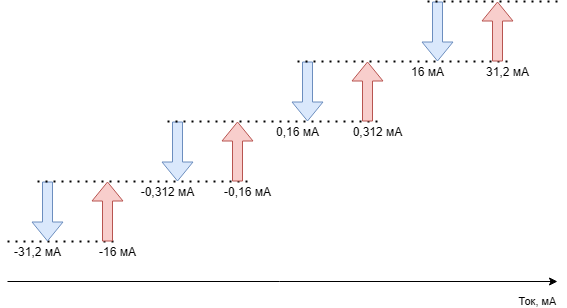
\includegraphics[scale = 0.55]{Shunts Level Switching.png}
    \caption{Уровни переключения шунтов}
    \label{ris:Shunts Level Switching}
\end{figure}

Данные пороговые значения соответствуют смещениям на 10 и 1950 отсчетов АЦП 
от <<центрального>> значения, определенного при калибровке устройства.

Агрегированные данные передаются в TCP-порт 21000 (выбран произвольно) 100 раз в секунду в виде 
усредненных значения потребляемого тока и накопленной мощности.

К командам, обрабатываемым Blackmagic, добавлены еще несколько для управления подсистемой питания 
и интерфейсом связи с отлаживаемым устройством, а кроме того, изменено поведение некоторых команд:

\begin{itemize}
    \item monitor tpwr [enable|disable] Включает и выключает сигнал запрета работы ST1S10
    \item monitor tpwr\_set [число] Устанавливает уровень напряжения на ST1S10
    \item monitor iface [enable|disable] Включает и выключает состояние Hi-Z на преобразователе 
    логических уровней
    \item monitor calibrate Выполняет калибровку АЦП (выполнять при нулевом потребляемом токе)
\end{itemize}

